%//cSpell:disable
% LTeX: enabled=false
\documentclass[a4paper,ngerman, headheight=28pt,12pt]{scrartcl}


% PACKAGES
\usepackage[a4paper,left=3cm,right=4cm,top=2.5cm,bottom=2.5cm]{geometry}

\usepackage{fontspec}
\usepackage{babel}
\usepackage{csquotes}
\usepackage{svg}
\usepackage{relsize}
\usepackage{setspace}

\usepackage{lineno}

\usepackage{tabularray}
\usepackage{float}

% Appendix
\usepackage{appendix}

% Title Spacing

\RedeclareSectionCommand[
  %runin=false,
  afterindent=false,
  beforeskip=.5\baselineskip,
  afterskip=.25\baselineskip]{section}
\RedeclareSectionCommand[
  %runin=false,
  afterindent=false,
  beforeskip=.25\baselineskip,
  afterskip=.125\baselineskip]{subsection}
\RedeclareSectionCommand[
  %runin=false,
  afterindent=false,
  beforeskip=.175\baselineskip,
  afterskip=.0625\baselineskip]{subsubsection}


% Literaturverzeichnis
\usepackage[
backend=biber,
style=alphabetic,
sorting=nty,
maxbibnames=99
]{biblatex}

\addbibresource{refs_facharbeit.bib}

\DeclareLabelalphaTemplate{
  \labelelement{
    \field[final]{shorthand}
    \field{label}
    \field[strwidth=2,strside=left,ifnames=1]{labelname}
    \field[strwidth=1,strside=left]{labelname}
  }
  \labelelement{
    \field[strwidth=2,strside=right]{year}
  }
}
%//TODO Change font back to calibri
%\setmainfont{Calibri}
\setmainfont{calibri}[
  Path=./fonts/,
  Extension=.ttf,
  UprightFont=*-Regular,
  BoldFont=*-Bold,
  ItalicFont=*-Italic,
  BoldItalicFont=*-BoldItalic,
]

\MakeOuterQuote{"}

\newcommand{\LongMinus}{–}

% LTeX: enabled=true
%//cSpell:enable
% Die nächsten vier Felder bitte anpassen:
\newcommand{\Titel}{Dezentralisierte asymmetrische \\ Verschlüsselung über Tor} % Titel für Facharbeit
\newcommand{\SubTitel}{Die Lösung für sicheres Messaging?}

\newcommand{\PageTitel}{Dezentralisierte asymmetrische Verschlüsselung \\ über Tor \LongMinus{} Die Lösung für sicheres Messaging?} % Seitentitel für Facharbeit
\newcommand{\Author}{Hendrik Lind}     % Ich
\newcommand{\Department}{Seminarfach Informatik}
\newcommand{\School}{Windthorst-Gymnasium Meppen}
\newcommand{\Country}{Deutschland}
\newcommand{\Abgabe}{20. November 2023}

\newcommand{\thesisDegree}{Facharbeit}
\newcommand{\faculty}{Seminarfach Informatik}
\newcommand{\thesisPlaceDate}{\today}

\newcommand{\vcite}[1]{\cite[vgl.][]{#1}}
\newcommand{\vebd}{[vgl. ebd.]}

% Tor Stuff
\newcommand{\entryn}{\textit{Entry Node\,}}
\newcommand{\relayn}{\textit{Relay Node\,}}
\newcommand{\relayns}{\textit{Relay Nodes\,}}
\newcommand{\exitn}{\textit{Exit Node\,}}
\newcommand{\exitns}{\textit{Exit Nodes\,}}
\newcommand{\nodes}{\textit{Nodes\,}}
\newcommand{\node}{\textit{Node\,}}
\newcommand{\onion}{\textit{Onion\,}}
\newcommand{\circuit}{\textit{Circuit\,}}
\newcommand{\circuits}{\textit{Circuits\,}}
\newcommand{\introp}{\textit{Introduction Point\,}}
\newcommand{\introps}{\textit{Introduction Points\,}}
\newcommand{\renp}{\textit{Rendezvous Point\,}}

% Implementation stuff
\newcommand{\identity}{\textit{Identity\,}}

%//cSpell:disable
% LTeX: enabled=false

% Kopf- und Fußzeilen
\usepackage{scrlayer-scrpage, lastpage}
\setkomafont{pageheadfoot}{\large\textrm}
\lohead{\PageTitel}
\rohead{\Author}
\cfoot*{\thepage{}/\pageref{LastPageDoc}}

% Position des Titels
\usepackage{titling}
\setlength{\droptitle}{-1.0cm}


% Für mathematische Befehle und Symbole
\usepackage{amsmath}
\usepackage{amssymb}
\usepackage{wrapfig}

% Für Bilder
\usepackage{graphicx}
\usepackage{graphbox}

% Für Algorithmen
\usepackage{algpseudocode}

% Für Quelltext
\usepackage{listings}
\usepackage{color}


\graphicspath{ {./img/} }


% 1.5 Line spacing
\setstretch{1.5}


% Defining rust langauge
\definecolor{GrayCodeBlock}{RGB}{241,241,241}
\definecolor{BlackText}{RGB}{110,107,94}
\definecolor{RedTypename}{RGB}{182,86,17}
\definecolor{GreenString}{RGB}{96,172,57}
\definecolor{PurpleKeyword}{RGB}{184,84,212}
\definecolor{GrayComment}{RGB}{170,170,170}
\definecolor{GoldDocumentation}{RGB}{180,165,45}
\lstdefinelanguage{rust}
{
    columns=fullflexible,
    keepspaces=true,
    frame=single,
    framesep=0pt,
    framerule=0pt,
    framexleftmargin=4pt,
    framexrightmargin=4pt,
    framextopmargin=5pt,
    framexbottommargin=3pt,
    xleftmargin=4pt,
    xrightmargin=4pt,
    backgroundcolor=\color{GrayCodeBlock},
    basicstyle=\ttfamily\color{BlackText},
    keywords={
        true,false,
        unsafe,async,await,move,
        use,pub,crate,super,self,mod,
        struct,enum,fn,const,static,let,mut,ref,type,impl,dyn,trait,where,as,
        break,continue,if,else,while,for,loop,match,return,yield,in
    },
    keywordstyle=\color{PurpleKeyword},
    ndkeywords={
        bool,u8,u16,u32,u64,u128,i8,i16,i32,i64,i128,char,str,
        Self,Option,Some,None,Result,Ok,Err,String,Box,Vec,Rc,Arc,Cell,RefCell,HashMap,BTreeMap,
        macro_rules
    },
    ndkeywordstyle=\color{RedTypename},
    comment=[l][\color{GrayComment}\slshape]{//},
    morecomment=[s][\color{GrayComment}\slshape]{/*}{*/},
    morecomment=[l][\color{GoldDocumentation}\slshape]{///},
    morecomment=[s][\color{GoldDocumentation}\slshape]{/*!}{*/},
    morecomment=[l][\color{GoldDocumentation}\slshape]{//!},
    morecomment=[s][\color{RedTypename}]{\#![}{]},
    morecomment=[s][\color{RedTypename}]{\#[}{]},
    stringstyle=\color{GreenString},
    string=[b]"
}
% end

% Umlaute erlauben
\lstset{literate=%
  {Ö}{{\"O}}1
  {Ä}{{\"A}}1
  {Ü}{{\"U}}1
  {ß}{{\ss}}1
  {ü}{{\"u}}1
  {ä}{{\"a}}1
  {ö}{{\"o}}1
}
%end


\definecolor{mygreen}{rgb}{0,0.6,0}
\definecolor{mygray}{rgb}{0.5,0.5,0.5}
\definecolor{mymauve}{rgb}{0.58,0,0.82}
\lstset{
  keywordstyle=\color{blue},commentstyle=\color{mygreen},
  stringstyle=\color{mymauve},rulecolor=\color{black},
  basicstyle=\footnotesize\ttfamily,numberstyle=\tiny\color{mygray},
  captionpos=b, % sets the caption-position to bottom
  keepspaces=true, % keeps spaces in text
  numbers=left, numbersep=5pt, showspaces=false,showstringspaces=true,
  showtabs=false, stepnumber=2, tabsize=2, title=\lstname{}
}
\lstset{language=Rust}          % Set your language (you can change the language for each code-block optionally)

% Diese beiden Pakete müssen zuletzt geladen werden
\usepackage[hidelinks]{hyperref} % Anklickbare Links im Dokument
\usepackage{cleveref}

% Für Code
\usepackage[outputdir=build]{minted}


% Titlepage required things


% Necessary packages for the titlepage:
\usepackage{tikz}
\usetikzlibrary{calc}
%\usepackage{graphicx}
% \usepackage{newtxtext}
%\usepackage{float}
\usepackage{comment}
% This command changes the font style where SLU promotes Arial
%\newenvironment{myfont}{\fontfamily{phv}\selectfont}{\par}


% Add line breaks to urls
\apptocmd{\UrlBreaks}{\do\f\do\m}{}{}
\setcounter{biburllcpenalty}{9000}% Kleinbuchstaben
\setcounter{biburlucpenalty}{9000}% Großbuchstaben

% Facharbeit

\begin{document}
% To add this template to the main.tex file, just add the command "% To add this template to the main.tex file, just add the command "% To add this template to the main.tex file, just add the command "\include{titlePageSLU} after "\begin{docuemnt}" in the main.tex file


% In this segment, enter the desired data to be shown at the title page
\newcommand{\thesisAuthor}{Firstname Lastname}
\newcommand{\thesisTitle}{Interesting Thesis Title}
\newcommand{\thesisSubTitle}{little bit more descriptive}
\newcommand{\thesisTitleTranslated}{Translated Headline}
\newcommand{\thesisDegree}{Master thesis project}
\newcommand{\university}{Swedish University of Argicultural Science, SLU}
\newcommand{\credits}{30 hp}
\newcommand{\faculty}{Faculty of blablabalba}
\newcommand{\thesisPlaceDate}{Place of puplication, Year}
\newcommand{\company}{Company name}

%------------------------------------------------------------------------------
\begin{titlepage}
\thispagestyle{empty}
\myfont

% Use this line of code if both SLU loggo and company/other institution loggo is desired. The positions are possible to change with the \hspace and \vspace syntax.
\begin{figure} [H]
\vspace{-3cm}
 \centering
\begin{minipage}[t]{.45\linewidth}
  \raggedright
  % Upload and include SLU loggo here:
  \hspace*{-2cm}
\includegraphics[width=\linewidth]{slu_logo_webb.png}
  
\end{minipage}%
  \begin{minipage}[t]{.45\linewidth}
  \vspace{-3.3cm}
 \raggedleft
% Upload and include other loggo here (loggo of wikipedia is used as an example):
 \hspace*{1cm}
\includegraphics[width =0.5\textwidth]{wikilogo.png} \hspace*{-1cm}
 
\end{minipage}
\end{figure}


% If only the logo for SLU is desired, delete "\begin{comment}" and "\end{comment}" to use this line of code:
\begin{comment}
\begin{figure}
\vspace{-3cm}
    \hspace*{-2cm}
\includegraphics[width = 0.3\textwidth]{slu_logo_webb.png}\hspace*{-2cm}
\end{figure}
\end{comment}


% Adds background picture. Delete code if no background picture is wanted.
\begin{tikzpicture}[overlay, remember picture]
\node[anchor=south west, 
      xshift=-0.2cm, 
      yshift=-0.2cm] 
     at (current page.south west)
     {
\includegraphics[width = 1.8\textwidth, height = 9cm]{background.png}}; 
\end{tikzpicture}


\vspace{1cm}
\par
\noindent
\Huge
\textbf{\thesisTitle}
\vspace{0.2cm}
\LARGE
\par
\noindent
- \thesisSubTitle\\
\rule[0.3cm]{\linewidth}{2pt}
\Large

% Delete this line if no translation is desired
\noindent
\textit{\thesisTitleTranslated}

\vspace{2cm}
\noindent
\LARGE
\thesisAuthor\\
\vspace{4 cm}
\small
\par \noindent
\thesisDegree $\cdot$ \credits
\par \noindent
\university
\par \noindent
\faculty
\par \noindent
\company
\par \noindent
\thesisPlaceDate

\end{titlepage}
 after "\begin{docuemnt}" in the main.tex file


% In this segment, enter the desired data to be shown at the title page
\newcommand{\thesisAuthor}{Firstname Lastname}
\newcommand{\thesisTitle}{Interesting Thesis Title}
\newcommand{\thesisSubTitle}{little bit more descriptive}
\newcommand{\thesisTitleTranslated}{Translated Headline}
\newcommand{\thesisDegree}{Master thesis project}
\newcommand{\university}{Swedish University of Argicultural Science, SLU}
\newcommand{\credits}{30 hp}
\newcommand{\faculty}{Faculty of blablabalba}
\newcommand{\thesisPlaceDate}{Place of puplication, Year}
\newcommand{\company}{Company name}

%------------------------------------------------------------------------------
\begin{titlepage}
\thispagestyle{empty}
\myfont

% Use this line of code if both SLU loggo and company/other institution loggo is desired. The positions are possible to change with the \hspace and \vspace syntax.
\begin{figure} [H]
\vspace{-3cm}
 \centering
\begin{minipage}[t]{.45\linewidth}
  \raggedright
  % Upload and include SLU loggo here:
  \hspace*{-2cm}
\includegraphics[width=\linewidth]{slu_logo_webb.png}
  
\end{minipage}%
  \begin{minipage}[t]{.45\linewidth}
  \vspace{-3.3cm}
 \raggedleft
% Upload and include other loggo here (loggo of wikipedia is used as an example):
 \hspace*{1cm}
\includegraphics[width =0.5\textwidth]{wikilogo.png} \hspace*{-1cm}
 
\end{minipage}
\end{figure}


% If only the logo for SLU is desired, delete "\begin{comment}" and "\end{comment}" to use this line of code:
\begin{comment}
\begin{figure}
\vspace{-3cm}
    \hspace*{-2cm}
\includegraphics[width = 0.3\textwidth]{slu_logo_webb.png}\hspace*{-2cm}
\end{figure}
\end{comment}


% Adds background picture. Delete code if no background picture is wanted.
\begin{tikzpicture}[overlay, remember picture]
\node[anchor=south west, 
      xshift=-0.2cm, 
      yshift=-0.2cm] 
     at (current page.south west)
     {
\includegraphics[width = 1.8\textwidth, height = 9cm]{background.png}}; 
\end{tikzpicture}


\vspace{1cm}
\par
\noindent
\Huge
\textbf{\thesisTitle}
\vspace{0.2cm}
\LARGE
\par
\noindent
- \thesisSubTitle\\
\rule[0.3cm]{\linewidth}{2pt}
\Large

% Delete this line if no translation is desired
\noindent
\textit{\thesisTitleTranslated}

\vspace{2cm}
\noindent
\LARGE
\thesisAuthor\\
\vspace{4 cm}
\small
\par \noindent
\thesisDegree $\cdot$ \credits
\par \noindent
\university
\par \noindent
\faculty
\par \noindent
\company
\par \noindent
\thesisPlaceDate

\end{titlepage}
 after "\begin{docuemnt}" in the main.tex file


%------------------------------------------------------------------------------
\begin{titlepage}
\thispagestyle{empty}
% Use this line of code if both SLU loggo and company/other institution loggo is desired. The positions are possible to change with the \hspace and \vspace syntax.
\begin{figure} [H]
\vspace{-2cm}
 \centering
\begin{minipage}[t]{.45\linewidth}
  \raggedright
  % Upload and include SLU loggo here:
  \hspace*{-2cm}
\includegraphics[width=\linewidth]{wgm.png}
  
\end{minipage}%
  \begin{minipage}[t]{.45\linewidth}
  \vspace{-3.3cm}
 \raggedleft
% Upload and include other loggo here (loggo of wikipedia is used as an example):
 \hspace*{2cm}
\includegraphics[width =0.5\textwidth]{enkrypton.png} \hspace*{-1cm}
 
\end{minipage}
\end{figure}

% Adds background picture. Delete code if no background picture is wanted.
\begin{tikzpicture}[overlay, remember picture]
\node[anchor=south west, 
      xshift=-0.2cm, 
      yshift=-0.2cm] 
     at (current page.south west)
     {
\includegraphics[width = 1.8\textwidth, height = 9cm]{background.png}}; 
\end{tikzpicture}


\vspace{1cm}
\par
\noindent
\Huge
\textbf{\Titel}
\vspace{0.2cm}
\LARGE
\par
\noindent
\SubTitel\\
\rule[0.3cm]{\linewidth}{2pt}
\Large

\vspace{2cm}
\noindent
\LARGE
\Author\\
\vspace{4 cm}
\small
\par \noindent
\thesisDegree
\par \noindent
\School
\par \noindent
\faculty
\par \noindent
\thesisPlaceDate

\end{titlepage}
\tableofcontents
\setcounter{page}{0}
\thispagestyle{empty}
\vspace{0.5cm}
\pagebreak


%//cSpell:enable
% LTeX: enabled=true
\linenumbers{}
\modulolinenumbers[5]
\section{Einleitung}
%//SECTION Einleitung
Russland, China, Iran. In all diesen totalitären Staaten herrscht eine starke Zensur \vcite{AmnReport}. Rund 1,7 Milliarden Menschen sind allein nur in diesen drei Staaten von der Einschränkung der Meinungsfreiheit betroffen \vcite{UnPop}. Wie können Bürger
dieser Staaten ihre Meinung also verbreiten und andere Staaten auf
%//TODO hier staatskritisch ist falsches wort mir fällt aber das richtige nicht ein
staatskritische Probleme aufmerksam machen, ohne sich selber in Gefahr zu bringen?
%//!SECTION
%//SECTION Problemstellung
\\
%//TODO Hier nochmal nach einer anderen Quelle suchen, die passt nicht 100%ig
Bei herkömmlichen Messengern, wie WhatsApp, Signal und Co., braucht die Außenwelt die Telefonnummern der im totalitären Staat wohnenden Bürgern und Reportern, um diese zu kontaktieren. Allerdings könnte ein totalitärer Staat, sich als Empfänger ausgeben, sodass Bürger/Reporter ihre private Nummer an den Staat überreichen und dieser somit jene Nummer rückverfolgen kann \vcite{LocPolice}.
Und genau hier liegt das Problem: Bürger und Reporter können nicht durch alltägliche Messenger mit der Außenwelt kommunizieren, da der Staat deren Nummer zurückverfolgen kann und somit weiter die Meinungsfreiheit einschränkt und unterbindet \vebd.
\\
Durch die zentrale Infrastruktur, welche die meisten Messenger, wie zum Beispiel WhatsApp und Signal verwenden, ist es für totalitäre Staaten, wie China, möglich, die IP-Adressen jener Server zu blockieren und somit für Bürger und Reporter unzugänglich zu machen \vcite{ChinaFirewall,CentralizedWhatsapp}.
\\
%//!SECTION
%//SECTION Lösungsvorschlag / Ziel
Ein dezentralisierter Messenger, welcher Ende-zu-Ende verschlüsselt ist und über das Tor-Netzwerk kommuniziert, könnte bei diesen Problemen eine Lösung sein. Die Frage, ob ein solcher Messenger die Lösung für Bürger eines totalitären Staates ist, soll in dieser Arbeit geklärt werden.
%//!SECTION
\\
%//SECTION E2EE Überleitung zu Kapitel-Auflistung
Um diese Frage beantworten zu können, beschäftigt sich diese Arbeit in dem zweiten Kapitel mit der asymmetrischen Verschlüsselung, welche benötigt wird um die Ende-zu-Ende-Verschlüsselung (E2EE) umzusetzen und die Definition der E2EE, sowie der Sicherheitsbetrachtung der asymmetrischen Verschlüsselung \vcite{E2EE-Method}. Die Arbeit geht dabei nicht auf weitere Padding-Verfahren ein.
Eine mögliche Lösung, um eine Anonymität über das Internet zu gewährleisten wird in Kapitel drei vorgeschlagen, wobei das Tor-Netzwerk eine wichtige Rolle spielt.
Diese Arbeit befasst sich im vierten Kapitel mit einer Dezentralisierung der Infrastruktur, um eine weitere Sicherheitsebene zu schaffen.
Zuletzt werden im fünften Kapitel die Vor- und Nachteile eines solchen Messengers betrachtet, im sechsten Kapitel wird eine mögliche Umsetzung des Messengers beschrieben und im siebten Kapitel wird ein Fazit gezogen.
%//!SECTION


\section{Asymmetrische Verschlüsselung}
%//SECTION E2EE und asymmetrische Verschlüsselung
Um einen sicheren Nachrichtenaustausch zu gewährleisten, wird in dieser Arbeit die E2EE implementiert. Bei der E2EE wird von dem Sender die Nachricht, bevor sie an den Empfänger geschickt wird, verschlüsselt \vcite{E2EE}. Dazwischenliegende Akteure, wie zum Beispiel Server oder mögliche Angreifer, können demzufolge die Nachricht nicht lesen \vebd. \textbf{Nur} der Empfänger der Nachricht kann diese auch entschlüsseln. Als Ent- und Verschlüsselungsverfahren der Nachrichten wird die asymmetrische Verschlüsselung verwendet \vebd. Diese Arbeit beschränkt sich bei der asymmetrischen Verschlüsselung auf das RSA-Verfahren.
%//!SECTION
\subsection{Grundlagen}
%//SECTION Grundlagen
Grundsätzlich gibt es bei der asymmetrischen Verschlüsselung ein Schlüsselpaar (Keypair), welches aus einem privaten Schlüssel (private key) und einem öffentlichen Schlüssel (public key) besteht \vcite{Rsa-Basics}. Diese beiden Schlüssel hängen mathematisch zusammen, sodass der öffentliche Schlüssel Nachrichten \textbf{nur} verschlüsseln aber nicht entschlüsseln kann \vebd. \textbf{Nur} der zum Schlüsselpaar dazugehörige private Schlüssel ist in der Lage, die verschlüsselte Nachricht wieder zu entschlüsseln (siehe \cref{fig:E2EE}) \vebd.

\begin{figure}[h]
  \centering
  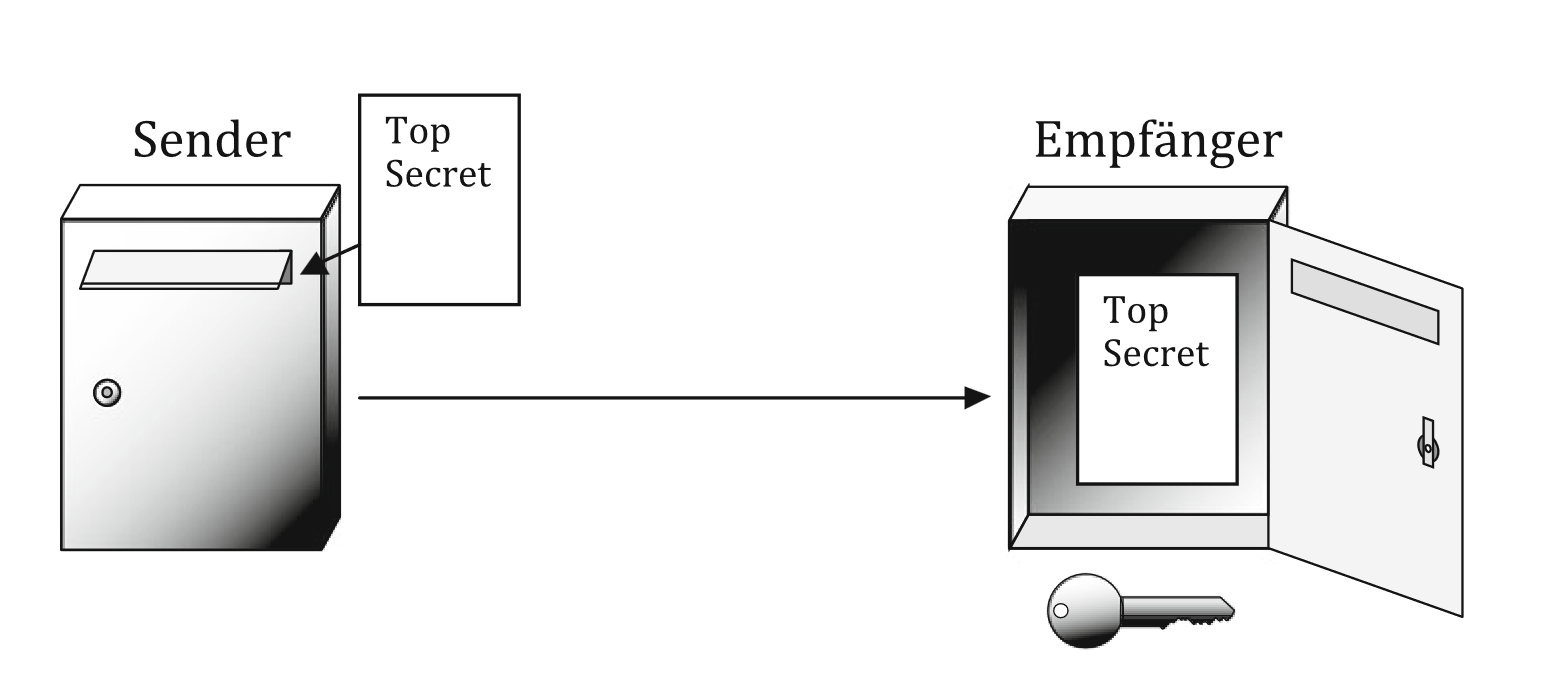
\includegraphics[width=0.75\textwidth]{Briefkasten-asymm.png}
  \caption{Jeder Sender kann mit dem öffentlichen Schlüssel die Nachricht "verschlüsseln" (also eine Nachricht in den Briefkasten werfen), aber nur der Empfänger kann den Briefkasten mit seinem privaten Schlüssel öffnen und somit die Nachricht herausnehmen\vcite{fig:Rsa-Cryptography} \label{fig:E2EE}}
\end{figure}
%//!SECTION

%//SECTION - Mathematische Betrachtung zu RSA
\subsection{Mathematische Betrachtung}
Alle Variablen der folgenden Berechnungen liegen im Bereich $\mathbb{N}$ \vcite{RsaGenCond}. \\
Für die Generierung des Schlüsselpaares benötigen wir zuerst zwei große zufällige Primzahlen, $P$ und $Q$ \vebd. Daraus ergibt sich $n = P * Q$, wobei $P \neq Q$, sodass $P$ bzw. $Q$ nicht durch $\sqrt{n}$ ermittelt werden kann \vebd. Der private Schlüssel besteht aus den Komponenten $\{ n, d \}$ währenddessen der öffentliche Schlüssel aus $\{ n, e \}$ besteht \vcite{RsaVariables}.
%//!SECTION
%//SECTION - Eulersche Phi-Funktion
\subsubsection{Eulersche Phi-Funktion}
Die Eulersche Phi-Funktion spielt eine wichtige Rolle in dem RSA-Verfahren \vcite{TotientFuncMultiplicative}. Grundsätzlich gibt $\phi(x)$ an, wie viele positive teilerfremde Zahlen bis $x$ existieren (bei wie vielen Zahlen der größte gemeinsamer Teiler ($\gcd$) $1$ ist) \vcite{EulersTotientFunction}. Somit ergibt $\phi(6) = 2$  oder bei einer Primzahl $\phi(7) = 7 - 1 = 6$ somit $\phi(x) = x-1$, wenn $x$ eine Primzahl ist, da jede Zahl kleiner als $x$ teilerfremd sein muss \vcite{TotientFuncMultiplicative}.
\begin{equation*}
  \begin{aligned}
    \phi(n) & = \phi(P \cdot Q)                                                \\
    \phi(n) & = \phi(P) \cdot \phi(Q)                                          \\
    \phi(P) & = P -1                                          & \phi(Q) = Q -1 \\
    \phi(n) & = \left(P - 1 \right) \cdot \left( Q - 1\right)
  \end{aligned}
\end{equation*}
%//!SECTION
\subsubsection{Generierung des Schlüsselpaares}
Sowohl der private als auch der öffentliche Schlüssel besteht unter anderem aus folgender Komponente: $n = P \cdot Q$ \vcite{RsaMaths1}.
Für den öffentlichen Schlüssel benötigen wir die Komponente $e$, die zur Verschlüsselung einer Nachricht verwendet wird \vebd. $e$ ist hierbei eine zufällige Zahl, bei welcher folgende Bedingungen gelten \vebd:
\begin{equation*}
  e = \begin{cases}
    1 < e < \phi(n)      \\
    \gcd(e, \phi(n)) = 1 \\
    \text{$e$ kein Teiler von $\phi(n)$}
  \end{cases}
\end{equation*}
Mit der errechneten Komponente $e$, welche Nachrichten verschlüsselt, kann der öffentliche Schlüssel nun an den Sender übermittelt werden.

Um den privaten Schlüssel zu berechnen, benötigen wir die Komponente $d$, welche zur Entschlüsselung verwendet wird \vcite{RsaEncryptionDecryption}.
\begin{equation*}
  \begin{aligned}
    \phi(n)   & = (P-1)(Q-1)     \\
    e \cdot d & = 1 \mod \phi(n)
  \end{aligned}
\end{equation*}

\subsection{Sicherheit}
Um die Sicherheit des RSA-Verfahrens betrachten zu können, müssen wir nun den Ver-/Entschlüsselungsvorgang betrachten.
\begin{equation*}
  \begin{aligned}
    c & = m^e \mod n & \text{Verschlüsselung zu $c$ mit $m$ als Nachricht}    \\
    m & = c^d \mod n & \text{Umkehroperation (Entschlüsslung) von $c$ zu $m$}
  \end{aligned}
\end{equation*}
Um die verschlüsselte Nachricht $c$ zu entschlüsseln, bräuchte ein Angreifer die Komponente des privaten Schlüssels $d$. $d$ ist allerdings mit einem starken Rechenaufwand verbunden, da, wie schon vorher bereits gezeigt, dafür $\phi(n)$ kalkuliert werden müsste. Somit wird eine Primfaktorzerlegung von $n$ benötigt wird \vcite{EulersTotientFunction}. Bei der Verschlüsselung von $m$ zu $c$ liegt eine Trapdoor-Einwegfunktion vor \vcite{RsaTrapdoor}. Das bedeutet, dass es zwar leicht ist $f(x) = i$ zu berechnen (bei RSA: Verschlüsselung), es jedoch unmöglich ist von $i$ auf den Ursprungswert $x$ zu schließen, ohne dass weitere dafür notwendigen Komponente bekannt sind (bei RSA wäre die benötigte Komponente $d$) \vebd.
\begin{figure}[h]
  \centering
  \includesvg[width=0.5\textwidth]{img/Trapdoor_permutation.svg}
  \caption{Die Trapdoor-Einwegfunktion bildlich dargestellt\vcite{fig:TrapdoorPermutation} \label{fig:TrapdoorFunc}}
\end{figure}

Wichtig bei dem RSA-Verfahren ist, dass die Länge von $n$ (die Schlüssellänge) mindestens 3000 Bit betragen sollte, da sonst die Primfaktorzerlegung von $n$ mit modernen Computern möglich sein könnte \vcite{RsaKeyLength}.

%/REVIEW - Ist das wirklich nötig? Oder kann ich mir das sparen? (ja schon)
\subsection{Vergleich zur symmetrischen Verschlüsselung}
Bei der symmetrischen Verschlüsselung wird der gleiche Schlüssel sowohl für die Verschlüsselung als auch für die Entschlüsselung verwendet \vcite{GeneralSymmetricCryptography}.
%/REVIEW - Wirklich padding mit einbeziehen? (meinte er brauch ich nicht)
Im Vergleich zu der asymmetrischen Verschlüsselung, ist die symmetrische Verschlüsselung schneller und keine Beschränkung des Chiffretextes \vcite{RsaAESAnalysis, OpensslRsaMaxLength}. Jedoch muss der Schlüssel der symmetrischen Verschlüsselung sicher an den jeweils anderen Kommunikationspartner übermittelt werden, um Nachrichten zu entschlüsseln \vebd.

\section{Das Tor-Netzwerk}
Die Anonymität des Messengers ist ein weiterer zentraler Aspekt, um die jeweiligen Kommunikationspartner zu schützen. Das Tor-Netzwerk ist hierbei ein möglicher Lösungsansatz, da normalen Routing, wie wir es tagtäglich nutzen, der Client kommuniziert  direkt mit dem Zielserver, somit der Zielserver die IP-Adresse des Clients einsehen kann \vcite{TCP_IP}.
%//REVIEW für den Satz danach Quelle?
Eine Rückverfolgung der IP-Adresse ist somit möglich \vcite{LocPolice}. Und genau bei diesem Problem setzt das Tor-Netzwerk an. Das Tor-Netzwerk besteht hierbei aus vielen \nodes, welche eingehende Tor-Verbindungen akzeptieren und weiterverarbeiten. Damit ein Client eine Anfrage über das Netzwerk verschicken kann, sucht er zunächst einen Pfad durch das Netzwerk, genannt \circuit \vcite{TorCircuits}. Der \circuit besteht dabei meist aus drei \nodes und ist für 10 Minuten gültig, bis der Client das \circuit erneuert (also einen neuen Pfad "sucht")  \vcite{FAQCircuitLifetime}. Die drei \nodes werden klassifiziert in einer \entryn, einer \relayn und einer \exitn, worüber später Anfragen an die Zielserver geschickt werden können \vebd.
Dabei verschlüsselt der Client verschlüsselt die eigentliche Anfrage mehrmals, hüllt sie also in ein mehrere "Schalen" ein, welche eine \onion bilden, und leitet diese über den \circuit an den Zielserver weiter\vcite{TorDesign}. Anfangs wird die \onion von dem Tor-Client an die \entryn geschickt \vebd. Bei jeder \node, wie der \entryn, wird eine Schale der \onion "geschält" (die \onion also einmal entschlüsselt), welche Informationen zu dem nächsten Knotenpunkt enthält \vcite{TorStructure2}. Die Node leitet nun die um eine Schale "geschälte" \onion an den nächsten Knotenpunkt weiter \vebd.
Sobald die Anfrage bei der \exitn angekommen ist, entfernt diese die letzte "Schale" der Anfrage, welche nun vollständig entschlüsselt ist und an den Zielserver geschickt werden kann \vebd. Dieses Routing-Verfahren ist auch als \textit{Onion-Routing} bekannt \vcite{TorDesign}.

\begin{figure}[h]
  \centering
  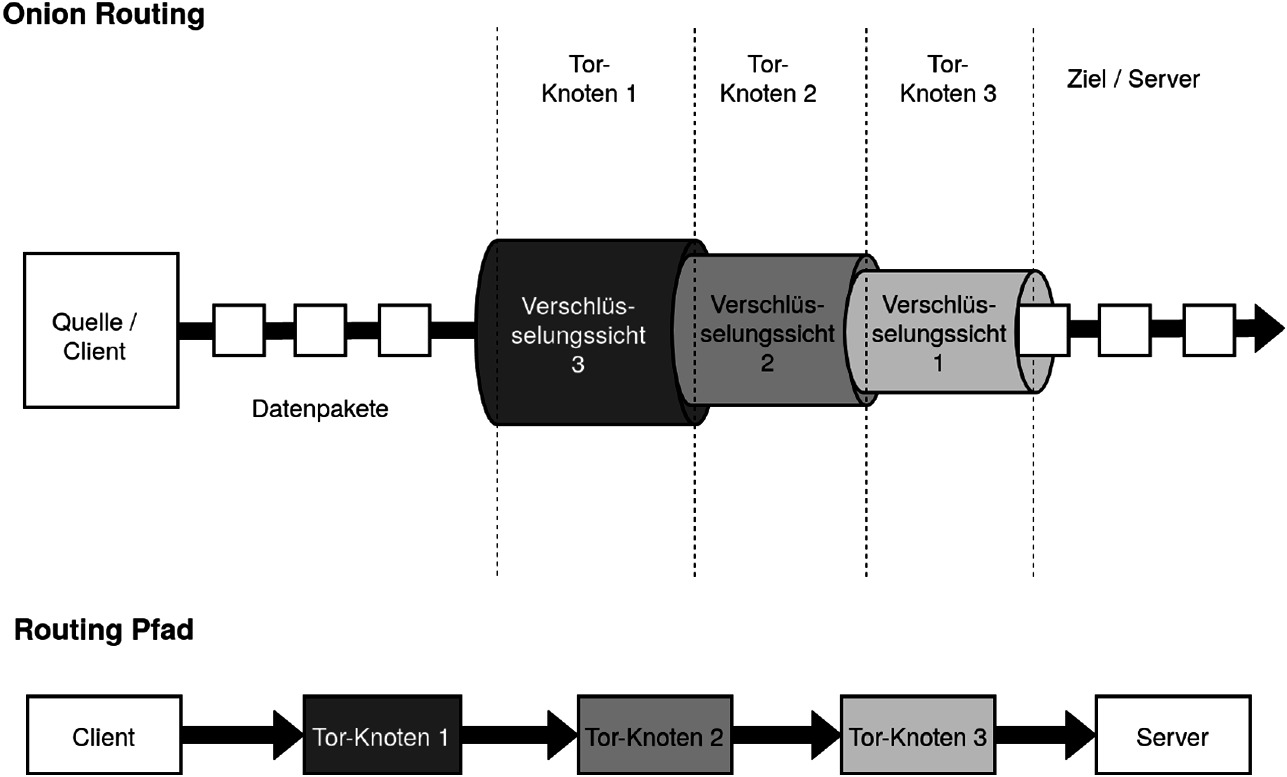
\includegraphics[width=0.65\textwidth]{TorRoutingSimple.png}
  \caption{Das Prinzip des Onion-Routings \vcite{fig:Tor-Structure} \label{fig:TorStructure}}
\end{figure}

%//TODO Checken ob das wirklich in der quelle so steht, sollte eig
\textbf{Nur} die \entryn weiß somit die reale IP-Adresse des Clients und \textbf{nur} die \exitn weiß, an welchen Zielserver die Anfrage geschickt wurde \vcite{TorStructure2}. Dazwischenliegende \nodes, wie die \relayn erkennen nur eine verschlüsselte Anfrage und haben keinerlei Informationen über den eigentlichen Client oder den Zielserver. Die \exitn schickt allerdings die Anfrage ohne Verschlüsselung des Tor-Netzwerkes an den Zielserver, wodurch Informationen der Nutzer ausgelesen werden könnten (wenn die Anfrage nicht über das HTTPS-Protokoll versendet wurde) und zusätzlich die IP-Adresse des Zielservers speichern \vcite{TorExitNodeVulnerability}. Durch Etablieren von \exitns in dem Tor-Netzwerk könnten Angreifer somit die Anonymität des Netzwerkes bzw. der Nutzer gefährden \vebd.

\subsection{Onion Services}
Onion Services sind eine mögliche Lösung für den \exitn-Angriff \vcite{TorOnionServiceTalk}. Diese nicht auf die \exitn angewiesen sind und agieren nur innerhalb des Tor-Netzwerkes mit anderen Tor-Clients und verhalten sich wie normale Tor-Clients \vebd. Onion Services sind nicht über das normale Internet erreichbar, wie die Zielserver im vorherigen Beispiel, sondern nur über das Tor-Netzwerk \vcite{TorOnionService}. Bei Onion Services müssen im Vergleich zu normalen öffentlichen Servern keine Ports geöffnet werden, damit ein Client sich mit dem Server verbinden kann, da der Onion Service direkt mit dem Tor-Netzwerk über ausgehende Verbindungen kommuniziert (auch bekannt als \textit{NAT punching}) und darüber sämtliche Daten geleitet werden \vebd.

%//NOTE bis hier überprüft

\subsubsection{Verbindungsaufbau}
Zunächst generiert der Onion Service ein Schlüsselpaar, bestehend aus einem öffentlichen und einem privaten Schlüssel \vcite{GeeksOnionService}. Unter anderem wird nun aus dem öffentlichen Schlüssel die Adresse des Onion Services generiert und endet mit ".onion" \vebd. Ein Beispiel für eine solche Adresse ist die der Suchmaschine DuckDuckGo: \\
\textit{duckduckgogg42xjoc72x3sjasowoarfbgcmvfimaftt6twagswzczad.onion} \vcite{DuckDuckGoLink}.
%/REVIEW sehr oft gleiche Quelle (L meinte is okay)
Der Onion Service sich nun mit dem Tor-Netzwerk wie ein normaler Client über einen \circuit, welcher aus drei \nodes besteht \vcite{TorOnionService}. Der Service sendet eine Anfrage an das letzte Relay im \circuit, sodass es als \introp dient und etabliert eine Langzeitverbindung jenem (der \circuit erneuert sich also nicht alle 10 Minuten wie bei dem Tor-Client) \vebd. Dieser Vorgang wiederholt sich zweimal, bis der Onion Service drei \introps auf drei verschiedenen \circuits gefunden hat \vebd. Damit andere Clients den Onion Service erreichen können, erstellt der Onion Service einen \textit{Onion Service descriptor}, welcher die Adressen der \introps und Authentifizierungsschlüssel enthält, signiert diesen mit seinem privaten Schlüssel und schickt den \textit{Descriptor} an die Directory Authority \vcite{TorSpecDerivingKeys, TorSpecDirectoryInf}. Die Directory Authority ist ein Server, welcher Informationen über das Tor-Netzwerk, wie zum Beispiel die des Onion Services, speichert und verteilt \vcite{TorDirectoryAuthority}. Im Sinne dieser Arbeit, hat der Onion Service sich nun von Person A mit dem Tor-Netzwerk verbunden, jedoch braucht es noch Person B, welche sich über ihren Tor-Client mit dem Onion Service der Person B verbindet. Damit der Tor-Client von Person A sich allerdings verbinden kann, fragt der Client nun die Directory Authority an den signierten \textit{Descriptor} des Onion Services von Person B an den Client zu schicken \vcite{TorStructure}. Der Client besitzt nun die Adressen der \introps und die Signatur des \textit{Descriptors}, sodass dieser mit dem öffentlichen Schlüssel der Onion Adresse die Signatur überprüfen kann \vebd. Der Client generiert nun 20 zufällige Bytes (Secret) und schickt diese an eine zufällig ausgewählte \relayn, welche nun als \renp dient \vcite{TorSpecRendezvous}. Das Secret wird von dem Client auch an eine von den \introps geschickt, sodass der Onion Service mit dem gleichen Secret eine Verbindung zu dem \renp aufbauen kann \vcite{TorSpecIntroP}. Der \renp leitet, wenn der Client und der Onion Service über deren \circuits miteinander verbunden sind, die Nachrichten zwischen den beiden weiter \vcite{TorSpecRendezvous}. Der Client und der Onion Service kommunizieren nun also nur über das Tor-Netzwerk miteinander und sind nicht mehr auf die \exitn angewiesen.

\subsection{Sicherheit}
%//TODO Nochmal Studio durchlesen, ist noch nicht schlüssig
%//TODO Angriff wurde schon von Tor gefixt, benutze OnionServiceFingerprinting
%//TODO Clearnet erklären
In der Sicherheitsbetrachtung beziehe ich mich ausschließlich auf die Verbindung zwischen Onion Services und Tor-Clients (also nicht zwischen Tor-Client und \exitn).

Das Tor-Netzwerk in Verbindung mit den Onion Services liefert, wie bereits erläutert, durch \circuits und \renp eine hohe Anonymität. Im Gegenzug sorgt die hohe Anonymität, welche durch die vielen \nodes und durch mehrfache Verschlüsselungen erreicht wird, auch dazu, dass das Tor-Netzwerk um das 120-fache langsamer ist im Vergleich zum normalen Routing \vcite{TorPerformance}.
Das Tor-Netzwerk ist praktisch unmöglich in der Praxis zu blockieren, da über 6.500 verschiedene \nodes existieren und es somit keinen zentralen Hauptserver gibt, von welchem das Tor-Netzwerk abhängig ist \footnote{Es ist zwar möglich die IP-Adressen jeglicher \relayns zu blockieren, jedoch ist dies durch Pluggable Transports umgänglich \vcite{PluggableTransports}} \vcite{DeanonymizingTorBook}.
Theoretisch ist eine Deanonymisierung eines Onion Services möglich, wenn der ISP (Internet Service Provider, also z.B. Telekom, EWE, etc.) eingehende und ausgehende Verbindungen zwischen Client und Onion Service bzw. zu deren \relayn aufzeichnet und diese mithilfe von Machine Learning analysiert \vcite{OnionServiceFingerprinting}. Dabei war die Umsetzung der theoretischen Grundlage bis jetzt mit idealisierten Bedingungen erfolgreich, jedoch braucht es noch weiterer Studien, um die möglichen Gefahren dieses Algorithmus einzustufen \vebd. Dabei könnten, wenn die deutsche, amerikanische und die französische Regierung zusammenarbeiten, 78,34 \% der \circuits deanonymisieren \vebd.
%//FIXME - Hier is irgend nen Kasus Fehler
Dieses Szenario erscheint jedoch unrealistisch, da Bürger in Deutschland, in den USA und in Frankreich ein Recht auf Meinungsfreiheit besitzen und höchstwahrscheinlich keine Deanonymisierungsangriff starten, um die Privatsphäre zum Beispiel von Whistleblowern zu schützen  \vcite{AmnReport,ROG-USA}.
%//TODO Später nochmal hier drauf eingehen, ist unrealistisch, dass die Regierungen zusammenarbeiten, um Meinungsfreiheit und Whistleblower unterdrücken.


\section{Dezentralisierung}
Mit den vorgeschlagenen Konzepten ist der Messenger imstande anonym (durch das Tor-Netzwerk und Onion Services) und sicher (durch asymmetrische Verschlüsselung) zu kommunizieren, jedoch wurde die Infrastruktur des Messengers noch nicht behandelt. Dafür ist die Betrachtung und Abwägung eines zentrales bzw. dezentrales Netzwerkes notwendig. \\
Ein zentrales Netzwerk, zum Beispiel das Netzwerk von WhatsApp oder Signal, besteht aus einem Hauptserver, welcher Daten verarbeitet und mit welchem sich Clients verbinden können \vcite{WhatsappCentralized,SignalCentralized, CentralizedDefinition}.
%//REVIEW - Dass der Client vertrauen muss ist angegeben, aber nicht dass er es nicht überprüfen kann
Der Client muss bei dieser Netzwerkstruktur dem Hauptserver "vertrauen" und kann nicht überprüfen, ob der Server von einem Hacker kompromittiert wurde \vcite{MessagingNetwork}. Dezentrale Netzwerke bestehen hingegen aus mehreren Servern, auf welche Rechenoperationen und oder Daten aufgeteilt werden \vcite{DecentralizedDefinition}.


\subsection{Sicherheit}
%//REVIEW - Muss ich hier wirklich noch sagen warum durch Kompromittierung Daten ausgelesen werden können? Bzw. die zentrale Angriffsfläche ist doch logisch oder?
Im Beispiel eines Messengers bietet ein zentrales Netzwerk den Hauptserver als mögliche Angriffsfläche an, sodass diese entweder durch DDoS-Angriffe außer Betrieb gesetzt werden kann oder durch Kompromittierung des Servers sowohl der Empfänger als auch der Sender der Nachrichten ausgelesen werden kann (in Form von Onion-Adressen)\vcite{BSI-DDoS}.
%//TODO - Satz bisschen scuffed, ausschalten nicht das richtige Wort.
Ein dezentrales Netzwerk mit einer Peer-to-Peer-Architektur\footnote{Peer-to-Peer bedeutet, dass jeder Knotenpunkt im Netzwerk sowohl Client als auch Server sein kann, welche bidirektional kommunizieren \vcite{PeerToPeerDef}} hat hingegen eine größere Angriffsfläche, wodurch mehrere Knotenpunkte des Netzwerkes kompromittiert werden müssen, um das Netzwerk ausschalten zu können \vcite{GeeksCenralizeDecentralized}.
%//REVIEW - Hier gibt es irgendwie keine Quellen, maybe einfach logisch?
Am Beispiel des Messengers, sollten nur Gesprächsteilnehmer Teil des Netzwerkes sein, um zu verhindern, dass ein Angreifer durch simples Beitreten des Netzwerkes die Onion-Adressen der Gesprächsteilnehmer auslesen kann.


\section{Umsetzung des Messengers}
Für die Umsetzung des Messengers habe ich mich für die Programmiersprache Rust entschieden, da Rust Memory Safe ist und zusätzlich eine hohe Performance bietet \vcite{RustSecurity}. Ein weiterer Vorteil der Programmiersprache Rust ist, dass sie in eine ausführbare Datei kompiliert werden kann, sodass keine weiteren Binaries, wie zum Beispiel bei Python, benötigt werden \vcite{RustCompile}. Zudem benutze ich das Framework Tauri, welches mir ermöglicht eine Benutzeroberfläche für den Messenger zu erstellen \vcite{RustTauri}. Tauri verbindet hierbei die Weboberfläche eines Browsers mit einem Rust-Backend, wobei Weboberfläche und das Backend miteinander kommunizieren können \vebd. Als Frontend des Messenger verwende ich React. Auf den Quellcode des Frontends werde ich nicht eingehen, da es nur für die Benutzeroberfläche zuständig ist, somit zum Beispiel keine Verschlüsselung / Verbindung zum Tor-Netzwerk etc. stattfindet. \\
Das Backend habe ich in 7 Bibliotheken aufgeteilt: \textit{encryption} für die Verschlüsselung der Nachrichten, \textit{messaging} für die Kommunikation zwischen Knotenpunkten, \textit{payloads} für die verschiedenen Netzwerkpakete, welche zwischen Knotenpunkten verschickt werden, \textit{secure-storage} als eine generelle Bibliothek mit Generics, sodass beliebiges Struct symmetrisch verschlüsselt / gespeichert werden kann, \textit{storage-internal} welches die Implementierung der \textit{secure-storage} Bibliothek enthält, \textit{shared} für gemeinsame Funktionen und Konstanten, \textit{tor-proxy} für die Verbindung zum Tor-Netzwerk. \\
Da die Messenger mit einer Peer-to-Peer-Verbindung miteinander verbunden sind, muss jeder Messenger in der Lage sein sowohl als Client als auch als Server (in Form eines Onion Services) zu agieren.
\subsection{Peer-to-Peer-Verbindung}
Somit startet jeder Messenger einen HTTP-Server, welcher einen HTTP-Endpunkt anbietet (in diesem Messenger \textit{/ws/}), um eine Websocket\footnote{%//TODO Hier richtig zitieren
Ein Protokoll für bidirektionale Kommunikation zwischen Server und Client über HTTP \vcite{WebsocketDef}}-Verbindung aufzubauen. Der Server ist hierbei also in der Lage sowohl Packets %//TOOD Packets noch erklären?
zu empfangen als auch zu senden.
\begin{minted}[breaklines]{rust}
HttpServer::new(|| {
    return App::new()
        // Return the default message to tell other clients that this server is actually alive
        .service(hello)
        // The websocket endpoint
        .route("/ws/", web::get().to(ws_index));
})
// Bind just to localhost and run
.bind(("127.0.0.1", CONFIG.service_port()))?
.run()
.await?;
\end{minted}

Analog dazu besitzt jeder Messenger auch einen Websocket-Client, welcher sich mit den anderen Messengern verbinden kann, sodass eine Peer-to-Peer-Verbindung entsteht. Der Client verbindet sich hierbei mit den anderen Messengern folgendermaßen:
\begin{minted}[breaklines]{rust}
/// `onion_hostname` is the onion address of the other messenger to connect to
pub async fn new(onion_hostname: &str) -> Result<Self> {
  // [...]
  let connect_host = onion_hostname.to_string();

  //[...]

  // The address which is used to connect to the websocket
  let onion_addr = format!("ws://{}.onion/ws/", connect_host);

  debug!("[CLIENT] Creating proxy...");

  // Creating the Socks5Proxy client which is used to connect to the tor network
  let proxy = SocksProxy::new()?;
  debug!("[CLIENT] Connecting Proxy...");
  let mut onion_addr = Url::parse(&onion_addr)?;
  onion_addr
      .set_scheme("ws")
      .or(Err(anyhow!("[CLIENT] Could not set scheme")))?;

  // Connecting to the destination host using the proxyy
  let sock = proxy.connect(&onion_addr).await?;

  //[...]
  // Connecting to the websocket with the client
  let (ws_stream, _) = tokio_tungstenite::client_async(&onion_addr, sock).await?;

  // [...]
}
\end{minted}

\subsection{Tor-Netzwerk}
Um den HTTP-Server nun als Onion Service in das Tor-Netzwerk einzubinden, benötigt der Messenger eine Verbindung zum Tor-Netzwerk. Zudem wird der Tor-Proxy gebraucht, um eine Verbindung zu den Onion Services anderen Messengern aufzubauen. Dies setze ich in der \textit{tor-proxy} Bibliothek um.
Um den Tor-Proxy zu konfigurieren, wird eine Tor-Konfigurationsdatei benötigt, welche unter anderem den Port des HTTP-Servers und des Tor-Proxys angibt:
\begin{minted}{rust}
/// Converts the configuration to a `torrc` file format
async fn to_text(&self) -> Result<String> {
    let data = PathBuf::from(self.data_dir());

    let geo_ip = data.clone().join("geoip");
    let geo_ip6 = data.clone().join("geoip6");

    #[allow(unused_mut)]
    let mut config = format!(
        "SocksPort {}
HiddenServiceDir \"{}\"
HiddenServicePort 80 {}
DataDirectory \"{}\"
GeoIPFile \"{}\"
GeoIPv6File \"{}\"",
        self.get_socks_host(),
        self.service_dir().to_string_lossy().replace("\\", "/"),
        self.get_hidden_service_host(),
        self.data_dir().to_string_lossy().replace("\\", "/"),
        geo_ip.to_string_lossy().replace("\\", "/"),
        geo_ip6.to_string_lossy().replace("\\", "/"),
    );

    //[...]

    Ok(config)
}
\end{minted}

Der Tor-Proxy wird folgendermaßen gestartet:
\begin{minted}{rust}
let mut child = Command::new(TOR_BINARY_PATH.clone());
child.args(["-f", &get_torrc().to_string_lossy()]);
child.current_dir(TOR_BINARY_PATH.parent().unwrap());
child.stdout(Stdio::piped());
child.stderr(Stdio::piped());
//[...]
let child = child.spawn()?;
\end{minted}

Der Messenger ist nun mit dem Tor-Netzwerk verbunden und wartet auf eingehende Verbindungen von anderen Messengern unter der Adresse des Onion Services.
\subsection{Nachrichtenaustausch}
Grundsätzlich liegen folgende Phasen des Nachrichtenaustausches vor:
\begin{itemize}
  \item \textbf{\identity verification}: Der Client übersendet seine Identität an den Server, welcher dieser nun überprüft, ob der Client tatsächlich der ist, für den er sich ausgibt. Danach übersendet der Server seine Identität an den Client. Dieser überprüft nun, ob der Server tatsächlich der ist, für den er sich ausgibt.
  \item \textbf{Nachrichten versenden}: Jetzt, wo beide Seiten ihre Identität überprüft haben und sicher sind, dass keine möglichen Angreifer die Verbindung fälschen könnten, ist der Client/Server bereit Nachrichten zu versenden
\end{itemize}
Generell gilt, dass der Messenger einen gemeinsamen Datenspeicher mit dem inneren Client und Onion Service teilt. In diesem werden die Chats zwischen den Gesprächsteilnehmern gespeichert. Der Datenspeicher besteht also aus einer \textit{HashMap} an Chat-Datensturkturen, wobei der Schlüssel der Empfänger-Onionadresse entspricht.
\begin{minted}[breaklines]{rust}
pub struct StorageChat {
  /// All messages sent to this receiver or received from this receiver
  //[...]
  pub messages: Vec<ChatMessage>,

  /// The public key which is used to encrypt messages when being sent to the receiver
  //[...]
  pub rec_pub_key: Option<PublicKey>,
  //[...]
  pub receiver_onion: String,
  /// Private key of this messenger used to decrypt the messages that are being received
  //[...]
  pub priv_key: PrivateKey,
}
\end{minted}
Jeder Chat enthält dabei das "eigene" Schlüsselpaar (\textit{priv\_key}), welches durch RSA generiert wird und den öffentlichen Schlüssel (\textit{rec\_pub\_key}) des Empfängers, mit welchem später die Nachrichten an den Empfänger verschlüsselt werden.

\subsubsection{Identity verification}
Um das Konzept der E2EE umzusetzen, muss der Sender einer Nachricht sicher sein, dass der Empfänger tatsächlich der ist, für den er sich ausgibt. Um dies zu erreichen verifizieren sich Client und Server mit einem \identity-Packet, welches den Hostname des Servers/Client, die Signatur des Hostnames (durch den privaten Schlüssel des Chats signiert) und den öffentlichen Schlüssel des Schlüsselpaares (vom Chat) enthält. Am Beispiel des Clients sucht dieser zunächst in den gespeicherten Chats nach der Onion-Adresse des Empfängers. Sollte der Eintrag nicht vorhanden sein, wird ein neuer Chat generiert (somit auch ein neues Schlüsselpaar generiert). Das Identitätspacket wird also folgendermaßen generiert:
\begin{minted}{rust}
async fn identity(receiver: &str) -> Result<Self> {
  // Get the own hostname
  let own_hostname = get_service_hostname(true)
      .await?
      .ok_or(anyhow!("Could not get own hostname"))?;

  // Get the private key for the receiver (used to decrypt messages)
  let priv_key = StorageManager::get_or_create_private_key(receiver).await?;
  let pub_key = priv_key.clone().try_into()?;

  // Creating a signature for the receiver with the hostname
  let keypair = PKey::from_rsa(priv_key.0)?;
  let mut signer = Signer::new(*DIGEST, &keypair)?;

  signer.update(own_hostname.as_bytes())?;
  let signature = signer.sign_to_vec()?;

  // Return the identity packet
  Ok(C2SPacket::SetIdentity(Identity {
      hostname: own_hostname,
      signature,
      pub_key
  }))
}
\end{minted}

Der Client übersendet dieses Identitätspacket an den Server, welcher jenes Packet durch den gespeicherten öffentlichen Schlüssel (\textit{rec\_pub\_key}) des (aus seiner Sicht) Empfängers überprüft. Sollte die Signatur nicht valide sein, wird die Verbindung abgebrochen. Folgender Quellcode wird verwendet, um die Identität des Clients zu überprüfen:
\begin{minted}[breaklines]{rust}
async fn verify(&self) -> Result<()> {
  //[...]
  // Check if there is a public key for the given receiver
  let local_pub_key = STORAGE.read().await.get_data(|e| {
      let key = e.chats.get(remote_host)
          .and_then(|e| e.rec_pub_key.clone());

      return Ok(key)
  }).await?;

  debug!("Done");

  // If there is a public key, verify the signature
  if let Some(local_pub_key) = local_pub_key {
    info!("Verifying for hostname: {:?}", remote_host);
    let keypair = PKey::from_rsa(local_pub_key.0)?;
    let mut verifier = Verifier::new(*DIGEST, &keypair)?;

    // Verify the signature with the public key
    verifier.update(remote_host.as_bytes())?;
    let is_valid = verifier.verify(&signature)?;

    if !is_valid {
        warn!("[INVALID_SIGNATURE] Wrong signature was given! This may be an attack!");
        return Err(anyhow!("Wrong signature was given! This may be an attack!"));
    }

    //[...]
  } else {
    // Adding public key to storage because it does not exist
    //[...]
  }
  //[...]
}
\end{minted}
Falls die Identität valide ist, übersendet der Server seine eigene Identität an den Client. Der gleiche Vorgang der Validation findet nun auch auf dem Server statt. Wenn dieser die \identity als valide bestätigt, ist eine sichere Verbindung nun aufgebaut.
\subsection{Nachrichten versenden}
Wir gehen nun davon aus, dass der Client an den Server eine Nachricht versenden möchte. Er ruft nun zunächst den öffentlichen Schlüssel des Empfängers aus dem Datenspeicher ab und verschlüsselt die Nachricht. Anschließend übersendet er die verschlüsselte Nachricht an den Server.
\begin{minted}[breaklines]{rust}
/// Sends a message to the receiver with the given date and msg, internal function
async fn inner_send(&self, msg: &str, date: u128) -> Result<()> {
  let raw = msg.as_bytes().to_vec();

  let tmp = self.receiver_host.clone();
  debug!("Reading public key for {}...", tmp);

  // Firstly we need to get the public key of the receiver
  let pub_key = STORAGE
    .read()
    .await
    .get_data(|e| {
      e.chats
        .get(&tmp)
        .and_then(|e| e.rec_pub_key.clone())
        .ok_or(anyhow!("The pub key was empty (should never happen)"))
    })
    .await?;

  debug!("Sending");
  // And encrypt the message
  let bin = pub_key.encrypt(&raw)?;

  // And send it to the receiver, if we are the client, send a client packet if not, server packet
  match &*self.info.read().await {
    ConnInfo::Client(c) => {
      debug!("Client msg");
      let packet = C2SPacket::Message((date, bin));
      c.feed_packet(packet).await?;
    }
    ConnInfo::Server((_, s)) => {
      debug!("Server msg");
      let packet = S2CPacket::Message((date, bin));

      s.send(packet).await?;
    }
  };

  Ok(())
}
\end{minted}
Der Server empfängt über die Websocket-Verbindung die verschlüsselte Nachricht und entschlüsselt diese anschließend mit dem privaten Schlüssel des Chats.
\section{Nachteile und Lösungsmöglichkeiten}

\section{Fazit}

\pagebreak
\nolinenumbers{}
\printbibliography[notkeyword={figure}]
\label{LastPageDoc}

\pagebreak
\pagenumbering{arabic}% resets `page` counter to 1
\cfoot*{\roman{page}}
\appendix
\printbibliography[heading=subbibliography,title={Anhang},keyword={figure}]
Quellcode: \href{https://github.com/sshcrack/enkrypton}{https://github.com/sshcrack/enkrypton}

\end{document}
